\section{Application Scenarios}
IoT area covers a wide range of applications, and each of them can be varied from each other on system requirement.To better evaluate the capability of underlying ICN network, we need to design and deploy both classical and challenged IoT application scenario over ICN network. Therefore, we choose smart campus as a starting point, because it has a reasonable scale and most of the design can be easily fit into a larger scale scenario, such as smart city.
\subsection{Buidling Management System}
In the past decade, to solve the huge energy consumption issue and provide a intelligent building facility monitor and control service, building management system (BMS) has been developed and standardized  by both academia and industry. In a smart campus scenario, especially a campus as big as Rutger  University, BMS plays a significant role in taking control of a complex ecosystem such as climate control, security monitoring,smoke detection and so on. Most of these system running on heterogeneous communication protocol, and we will like to inter-connect them with homogeneous network protocol and enable the reachability by using name or identifier. 
\subsubsection{Architecture Design}
Given that BMS provides a User Interface for control operation and monitoring, but most of the traffic is generated by device self reporting, which means it is a data-producer-driven system.For example, thermostat adjustment is triggered by the fluctuated data reading from a temperature sensor and motion sensor will inform light switch when movement is detected. 

We classify the net devices into four types-- sensing device, core network device, BMS server, and actuating device. The sensing device here is the sink which has full network stack  and aggregates the data from wireless sensor network (WSN). In order to provide reachability of low power sensor and flexibility of sensor data retrieval, the sink maintains each sensor as an object or content. These objects can either be updated to BMS server by the sink directly, or be pulled by remote data consumer on demand. The actuating device is basically full-network-stack thermostat or light fixture, which provide a network interface for air conditioner or light bulb. The system architecture is shown as Figure~\ref{fig:bms_arch}. Environment monitoring service,occupation monitoring service and control service are running on BMS server to enable building automation. 

To simplify our system design, we refer to Building Automation and Control Network (BACnet) protocol~\cite{}, which has been standardized by  American Society of Heating, Refrigerating and Air Conditioning Engineers (ASHRAE), and applied in many commercial BMSs. Based on BACnet, we define the objects we mention above as the format shown in Table~\ref{}.Although BACnet is application layer protocol that requires middlleware to provide a mapping from name to specific network address(NA), we substitute the identifier with ICN name. The only difference between MF and NDN is the name field, where we use GUID and NDN name respectively. 
%change the icon of humity sensor, bulb, and AC. 
\begin{table}
\label{tab:bac_object}
\end{table}
\begin{figure}
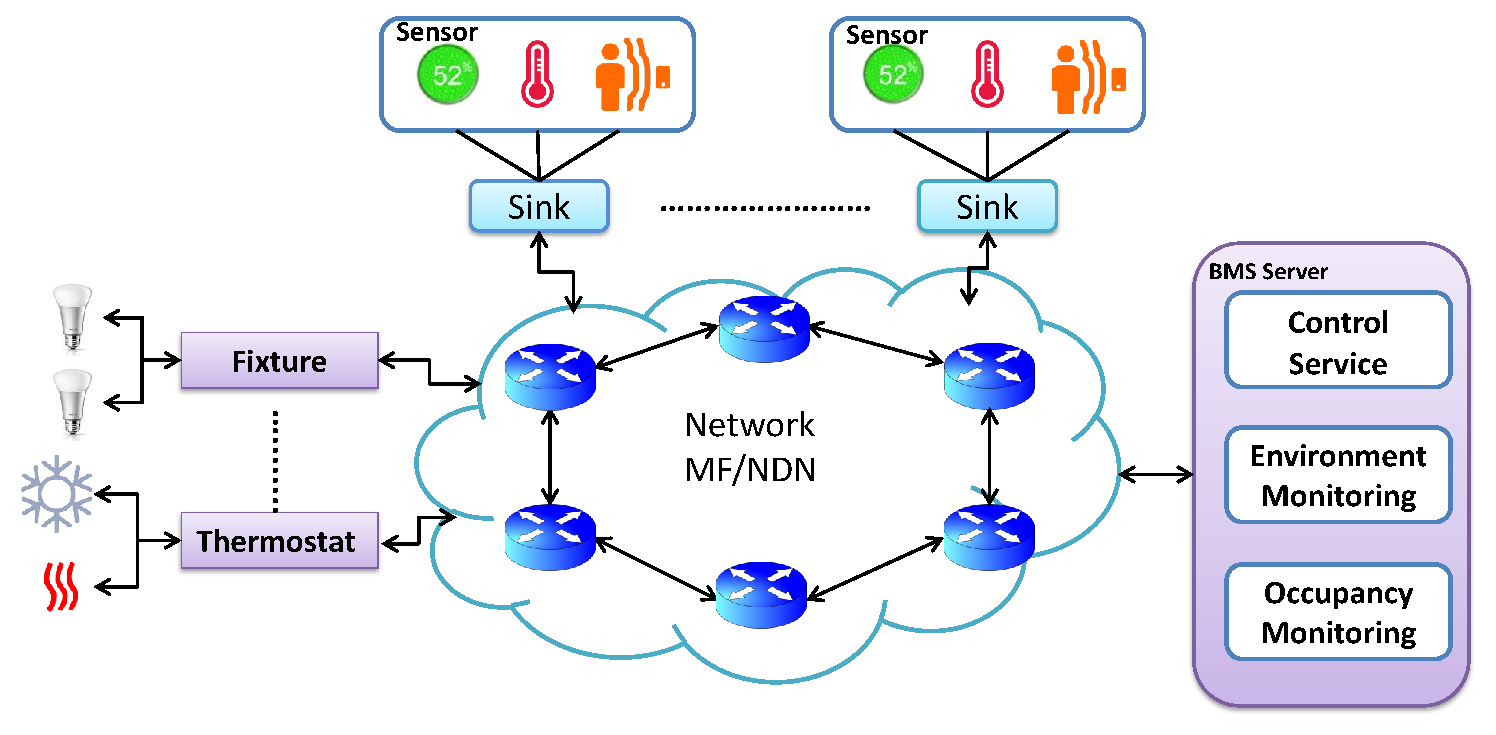
\includegraphics[width=3.1in,height=2.00in]{bms_arch.eps}
\caption{BMS over MF/NDN}
\label{fig:bms_arch}
\end{figure}
\subsubsection{One BMS Example of Device Discovery}
Since thousands of IoT devices are installed in buildings on campus, daily maintenance and configuration could be very complicated and time-consumed. With device discovery mechanism in MF, this task can be completed with less manual operation.

Assumed a new temperature sensor needs to be added to the big conference room in WINLAB, Rutgers University. It comes with a manufacturer serial number, which can also be used as its GUID (sensorGUID). The sink installed in this room is named with serviceGUID, representing service type "Environment Sensing". It connects to the nearest MF access router identified with rGUID, which stands for "Router@conferenceroom". As we discuss above, sensorGUID->serviceGUID mapping and sensorGUID->rGUID mapping will be inserted into GNRS server when the sink begins to receive message from the sensor. Configuration Service which periodically send look up for serviceGUID, and find the new device after comparing the result list with the local exiting devices list. As long as CS discover this new device, it exposes to the BMS server for further operation.
 
\subsection{School Bus System}
Another interesting scenario in a campus scenario is school bus system. It operates over the whole campus day and night, which thousands of students and faculties benefits from it. Now the increasing integration of sensors into vehicles makes a intelligent interactive school shuttle information system become possible.Specific applications such as fleet management system and NextBus system have been developed to provide a more efficient and convenient transportation service for the public. 

A smart bus system should provide network interfaces from vehicle  to infrastructure (V2I), and infrastructure to user.  Currently, the most common network device on bus is Mobile Data Terminal (MDT), which is a GSM-based communication module supporting data exchange between control center and bus via SMS. Most of vehicle support Controller Area Network bus (CANbus) protocol\cite{}. It enables sensors on vehicle can communicate with each other without a host computer. Also, sensor data such as velocity, seat occupation,and GPS obtained by CANbus can be transmit to the infrastructure via MDT directly. However, there are certain limitation on this type of communication model. First, SMS has constraint format of data, multimedia information from on-bus camera or microphone need to be transmitted in alternative way. Second, there is a significant delay from several seconds to several minutes via SMS per transmission, that make a real-time vehicle update become unrealistic. Since school bus operates in a wifi-covered campus, we assume that all shuttle routes are closed enough to the wifi access points. In a IP wifi network, given that the delay issue has been solved, mobility become a new challenge.Therefore, we propose a ICN infrastructure based school bus system (SBS) to evaluate the performance of both MF and NDN in dynamic environment.
\subsubsection{Architecture Design}
In our ICN based school bus system,  shown as Figure~\ref{},we dispose either MF Mobile Data Terminal(mMDT) or NDN (nMDT) Mobile Data Terminal on each bus respectively. To simplify our evaluation, we only choose three types of sensor which are relatively popular to user and system administrator -- velocity sensor, seat sensor, and GPS. Along with the bus route, enough number of access points are installed to provide seamless wifi coverage.Similar to our BMS design, a centralized SBS server handles updates from MDT, as well as sends notification to all buses or single bus. In order to support some specific application, we also need to evaluate the peer-to-peer communication in a V2I architecture. 
\begin{figure}
\includegraphics[width=3.1in,height=2.00in]{school_bus.eps}
\caption{Route A \& School Bus System Architecture}
\label{fig:bus}
\end{figure}
\subsubsection{Pub/Sub in The Same Route}
To give a example that combine both mobility and pub/sub in MF, we introduce a information sharing mechanism in the school bus system.  Supposed that drivers in Rutgers Bus Route A(shown in Figure~\ref{fig:bus}) interest in the position and occupancy of other buses among the same route. They subscribe to the "Route A Data Sharing from Bus\#1" service, and obtain a subscription GUID (subGUID) from server to listen.The access routers they attach will add this subGUID to the routing table and insert subGUID -> routerGUID mapping to the GNRS server.As the sender, Bus\#1 send position and occupancy information to the subGUID. If the packet arrives at the edge router, but the bus has moves to the next access point, the packet will be stored locally based on GSTAR protocol. The router then performs a GNRS lookup for for the latest NA (GUID of the access router) of the subGUID, and forward the packet to this NA.      
 
\subsection{Smart Parking System}